% Chapter 2

\chapter{Materials and methods} % Main chapter title
\label{Chapter2} % For referencing the chapter elsewhere, use \ref{Chapter2}

\bfseries{Cell line generation}\\
\normalfont Doxycycline-inducible wild-type and mutant GLUT1-expressing cell lines had been generated previously in the lab of Markus Landthaler at Max Delbr\"{u}ck Center. In brief, the gene \textit{SLC2A1} was purchased from Harvard Plasmid Repository and a stop codon was added with the primers listed in Table~\ref{tab:primers} (BioTeZ). The P485L mutation was introduced by PCR-directed mutagenesis with the primers listed in Table~\ref{tab:primers}. The wild-type and mutant \textit{SLC2A1} coding sequences were recombined into the vector pDEST-pcDNA5-BirA-FLAG using Gateway cloning system (ThermoFisher) (Figure~\ref{fig:vectors})~\cite{Couzens}. HEK293 Flp-In T-Rex cells (Invitrogen) were cotransfected with pOG44 Flp-recombinase expression vector (ThermoFisher) and the recombinant vector containing wild-type or mutant GLUT1 to generate stable cell lines. Two days following transfection, cells were selected with 100 \textmu g/mL Hygromycin B (InvivoGen) for 2 weeks. A control HEK293 cell line for BioID experiments had been generated in the lab using the identical technique with an integrated transgene for the inducible expression of the first 10 strands of GFP (GFP1-10).

\begin{table}[h]
%\captionsetup{font=normalsize}
\caption{Primer sequences for mutagenesis of GLUT1.}
\label{tab:primers}
\small
\centering
\begin{tabular*}{\textwidth}{l@{\extracolsep{\fill}}p{11.1cm}}
\toprule
\tabhead{Purpose} & \tabhead{Primer sequences (5' to 3')}\\
\midrule
Adding a stop codon & Forward: TCCCAAGTGTAATTGCCAACTTTCTTGTACAAAGTTG \newline Reverse: ATCAGCCCCCAGGGGATG\\
P485L mutation & Forward: CTGTTCCATCTCCTGGGGGCT \newline Reverse: CTCCTCGGGTGTCTTGTCAC\\
\bottomrule\\
\end{tabular*}
\end{table}
\begin{figure}[h]
%\captionsetup{font=normalsize}
\centering
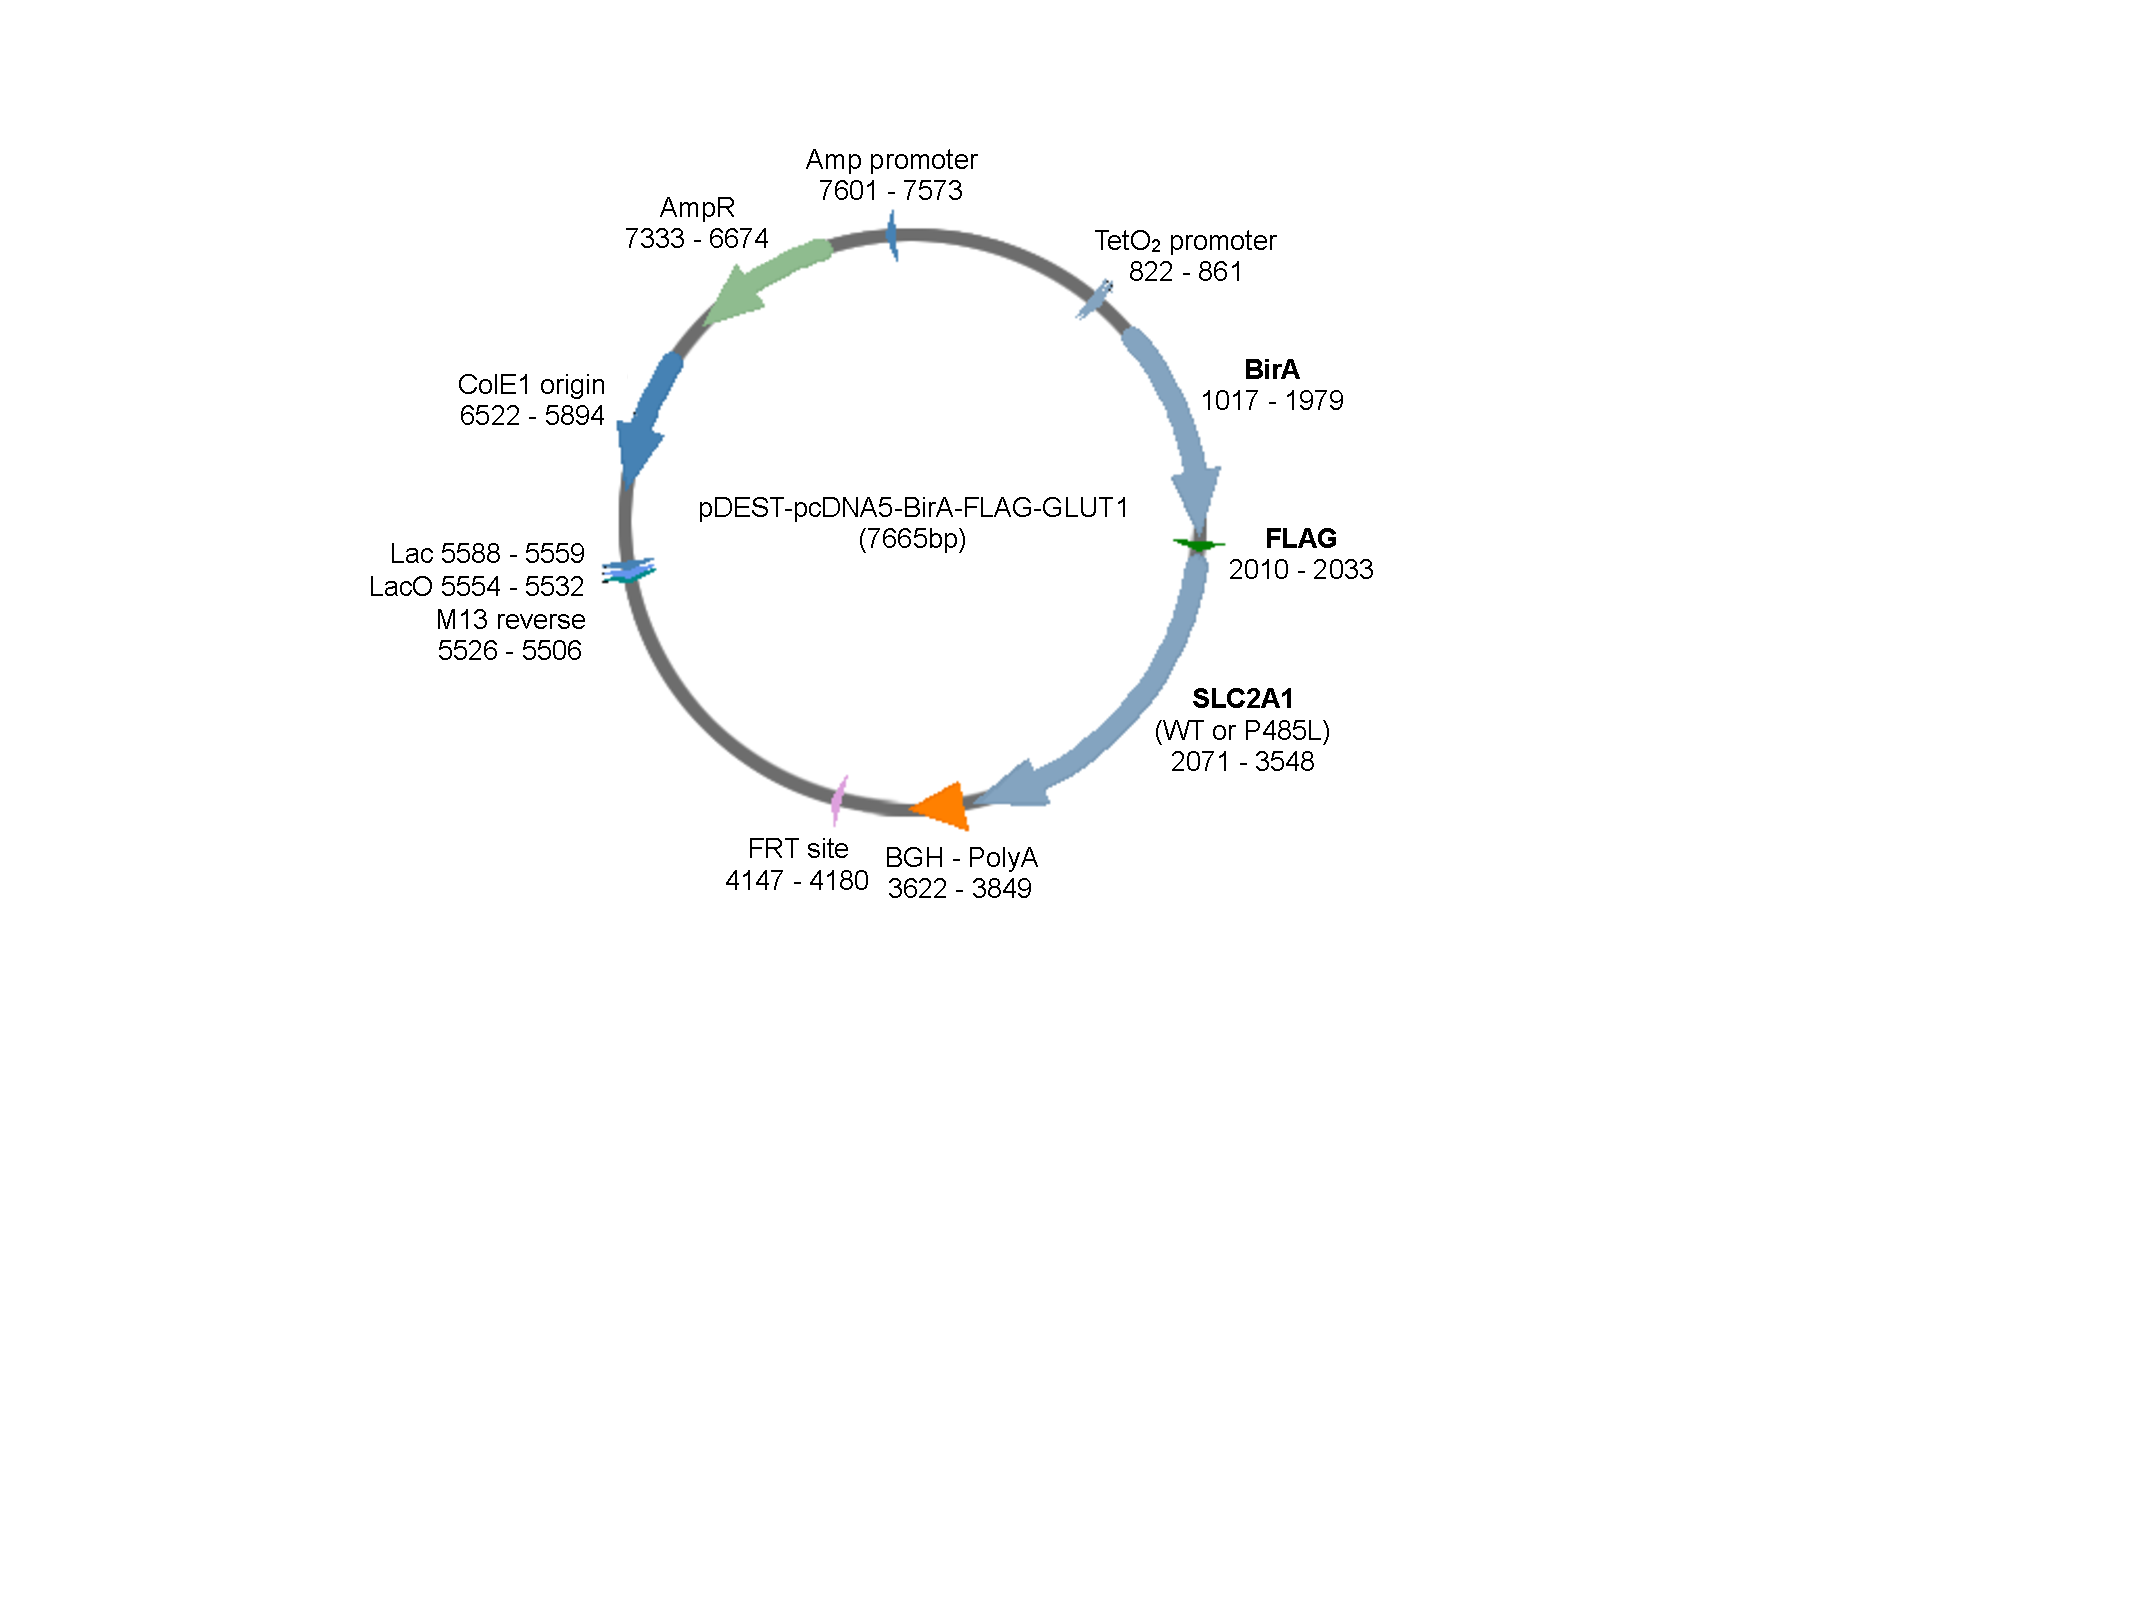
\includegraphics[scale=0.7]{Figures/vector}
\caption{Graphic map of the recombinant plasmid.}
\label{fig:vectors}
\end{figure}
The stable cell lines were stored in cryogenic vials (Croning) in liquid nitrogen. To recover cells, one vial of each cell line was warmed up to \SI{37}{\celsius} and the contents were diluted in 10 mL pre-warmed DMEM (Life Technologies) complemented with 10\% fetal bovine serum (Pan-Biotech). The medium is referred to as complete DMEM in the following. After spinning down at room temperature and 500 rpm for 3 min, the cell pellets were resuspended in 10 mL complete DMEM and seeded in T-75 flasks (CELLSTAR).
\\
\\*
\bfseries{Cell culture}\\
\normalfont Stable HEK293 cells were cultured at \SI{37}{\celsius} and 5\% CO\textsubscript{2} in culture flasks in complete DMEM. Cells were seeded to about 10\% confluency and routinely passaged twice a week as follows: the medium was aspirated and the cells were briefly washed with 4 mL sterile pre-warmed PBS (Life Technologies). To detach the cells 1 mL trypsin-EDTA (0.05\%, Life Technologies) was added and the flask was placed in an incubator at \SI{37}{\celsius} and 5\% CO\textsubscript{2} for 1 min. Trypsin was then inactivated with 9 mL pre-warmed complete DMEM. The medium was gently pipetted to the bottom of the flask in order to recover all the cells and get single-cell suspension. 1 mL of the cell suspension was transferred into 10 mL fresh complete DMEM in a new culture flask which was then placed back in the incubator. The cells would reach approximately 80\% confluency before the next passaging.

\begin{figure}[h]
\centering
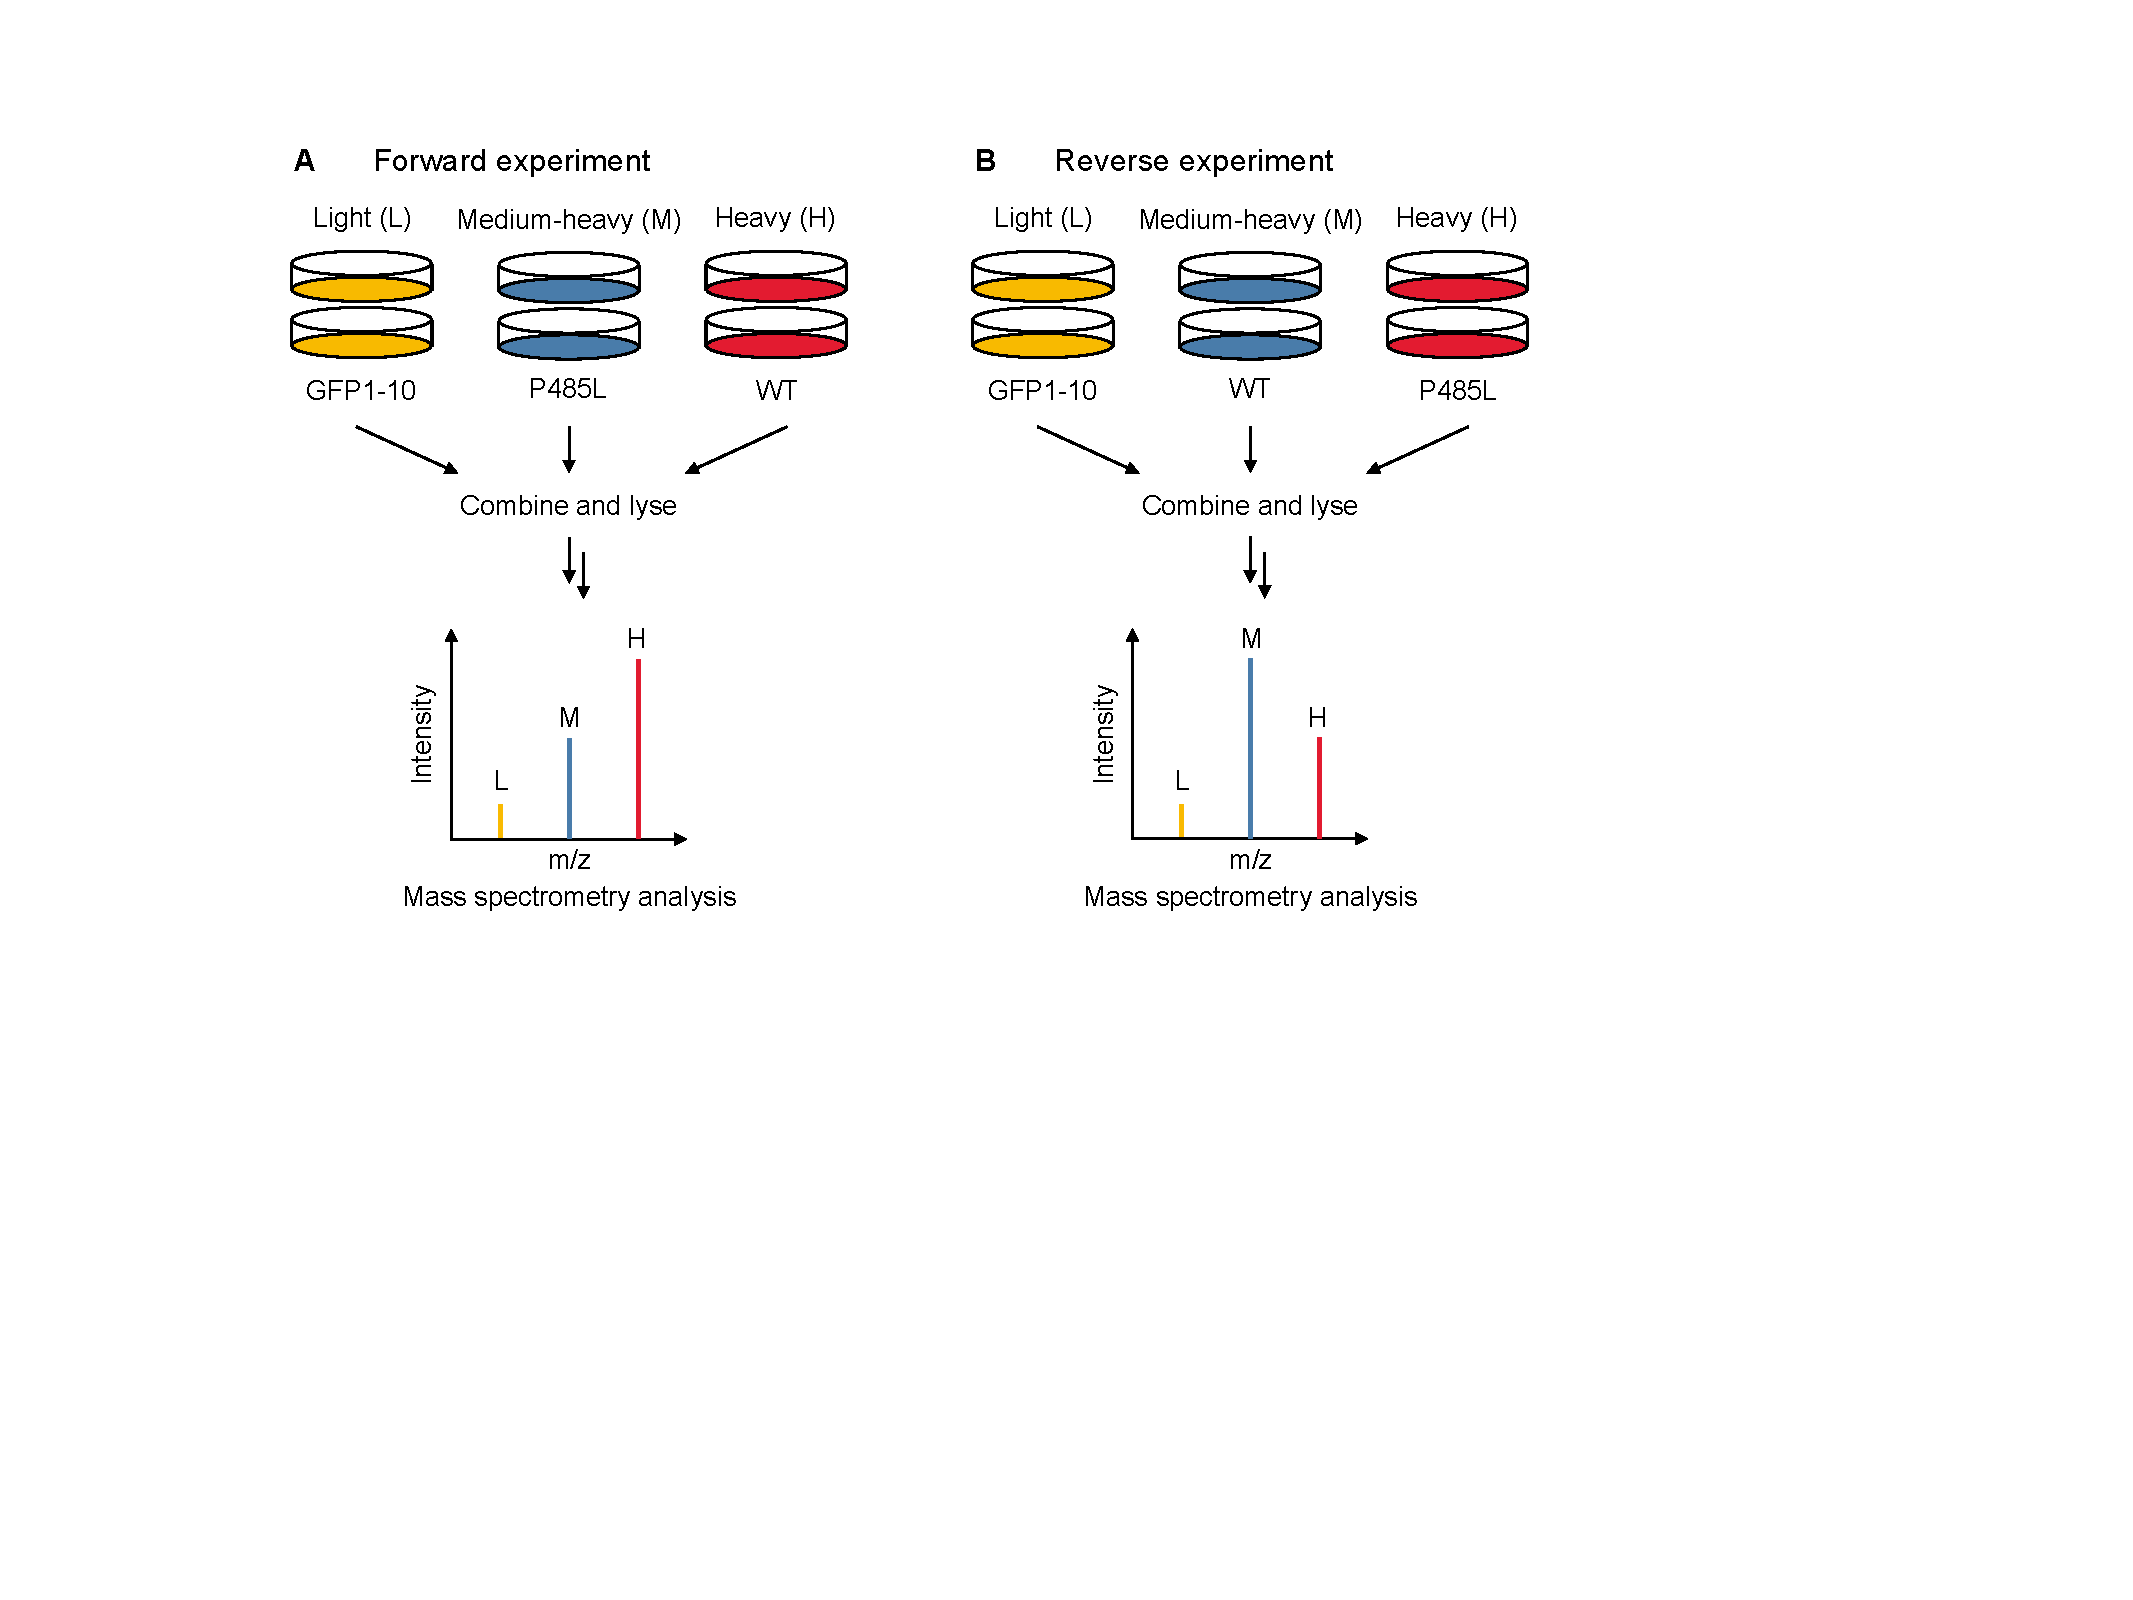
\includegraphics[scale=0.7]{Figures/BioID}
\caption{Experimental setup of triple SILAC labels.}
\label{fig:bioid}
\end{figure}
Cells used for BioID experiments were cultured in SILAC DMEM (Life Technologies) complemented with 2 mM glutamine (Glutamax, Life Technologies), 1 mM pyruvate (Life Technologies), 0.1 mM non-essential amino acids (Life Technologies) and 10\% dialyzed fetal bovine serum (Pan-Biotech). In addition, L-arginine (Arg0, Sigma-Aldrich) and L-lysine (Lys0, Sigma-Aldrich) were added to the Light SILAC DMEM to a final concentration of 0.199 mM and 0.339 mM, respectively. Alternatively, Arg6 and Lys4 or Arg10 and Lys8 were added in place of their Light counterparts to make Medium-heavy SILAC DMEM and Heavy SILAC DMEM, respectively. PBS-EDTA (Lonza) was used to detach the cells when passaging to avoid isotope contamination. After six passages cells were fully labeled as assessed by MS.
% From Koshi: stock conc. are Lys 0.798M, Arg 0.398M (my dilution is 1:2000). DMEM conc: Lys 146mg/L, Arg 84mg/L; if 1:3000 dilution, final conc. should be 1/4 of standard DMEM conc.

For the doxycycline induction experiments unlabeled HEK293 cells were cultured in 6-well plates. The cells were grown to approximately 50\% confluency on the second day after seeding. The medium was removed and 2 mL complete DMEM containing doxycycline (Sigma-Aldrich) was carefully added to each well. After 24 hr or 48 hr the cells were harvested for Western blotting analysis.

For the BioID experiments fully labeled HEK293 cells were seeded in 15 cm plates with approximately 25\% density. Two plates were used for each condition. HEK293 stable cells expressing GFP1-10 were labeled in Light SILAC DMEM and used as negative control cells. Besides the Light control cells, in the forward experiment mutant GLUT1 cells were cultured in Medium-heavy SILAC DMEM and wild-type GLUT1 cells were cultured in Heavy SILAC DMEM (Figure~\ref{fig:bioid} A), while in the reverse label-swap experiment wild-type GLUT1 cells were cultured in Medium-heavy SILAC DMEM and mutant GLUT1 cells were cultured in Heavy SILAC DMEM (Figure~\ref{fig:bioid} B). The cells were grown to 40\%-50\% confluency before being treated with 0.1 {}\textmu g/mL doxycycline and 1 mM biotin (ThermoFisher). After 24 hr, the cells were scraped in ice-cold PBS and collected for further BioID purification and MS analysis.

For the immunofluorescence experiments sterile glass coverslips (Roth, 18 mm diameter, 0.170 mm thickness) were placed in 12-well plates. Poly-L-lysine (0.01\%, Sigma-Aldrich) was added to each well to cover the coverslips. After incubation at room temperature for 5 min, poly-L-lysine was recovered from the wells and stored at \SI{4}{\celsius}. The coverslips were washed twice with sterile H\textsubscript{2}O before being air-dried completely. Unlabeled HEK293 cells were then seeded in the plates with approximately 25\% density. The cells were treated with 0.1 {}\textmu g/mL doxycycline on the second day and subjected to subsequent immunostaining on the third day.
\\
\\*
\bfseries{Western blotting}\\
\normalfont Cells were grown in 6-well plates as described above. After doxycycline or inhibitor treatment, cells were scraped in ice-cold PBS and spun down at 300 rcf, \SI{4}{\celsius} for 4 min. Cell pellets were lyzed for 15 min at room temperature in 100 \textmu L lysis buffer [50 mM ABC solution, 2\% SDS, supplemented with 60 Units/mL benzonase (Sigma-Aldrich) and protease inhibitors (Roche)]. Lysates were spun down at 16 100 rcf for 15 min to remove cell debris and supernatants were transferred to new Eppendorf tubes. For each SDS-PAGE sample, 15 {}\textmu L supernatant was diluted in LDS sample buffer (NOVEX) complemented with 1 {}\textmu L 1M DTT (Sigma-Aldrich) before being heated at \SI{70}{\celsius} for 10 min in a thermoblock. Samples were then loaded onto a 4\%-12\% gel (NOVEX) along with protein ladders (PageRuler Plus, ThermoFisher). Proteins were separated using electrophoresis for 90 min at 150 V in 400 mL MES running buffer (ThermoFisher). 

Before protein transfer a PVDF membrane (Merck Millipore) was activated in methanol for 1 min and equilibrated in ice-cold transfer buffer (25 mM Tris-HCl, 192 mM glycine, 20\% methanol, pH 8.3) for 10 min. Whatman filter papers and sponges were also soaked in transfer buffer for 10 min. A tank blotting system (Invitrogen) was used to transfer the separated proteins to the membrane. In short, a transfer sandwich was prepared with the membrane on the cathode and the gel on the anode. Air bubbles between the gel and membrane were removed by rolling them out with a roller. The cassette was then placed in the transfer tank on ice and the proteins were transferred at a constant current of 250 mA for 2 hr.

After protein transfer the membrane was blocked in 5\% milk powder in TBST (150 mM sodium chloride, 20 mM Tris-HCl, 0.1\% Tween-20, pH 7.6) at room temperature for 30 min. The membrane was then incubated with the primary antibody diluted in blocking buffer while rotating at \SI{4}{\celsius}. The membrane was washed 3 times for 5 min in TBST before being incubated at room temperature for 1 hr with the HRP-conjugated secondary antibody diluted in blocking buffer. The membrane was washed again before the chemiluminescence substrate (PerkinElmer) was applied to the membrane. The chemiluminescent signals were captured using a ChemiDoc MP Imaging System (Bio-Rad) and quantified with Image Lab 5.2.1. The primary and secondary antibodies used in this thesis are summarized in Table~\ref{tab:antibodies}.
\begin{table}[h]
\caption{Antibodies used for Western blotting and their dilutions.}
\label{tab:antibodies}
\small
\centering
\begin{tabular*}{\textwidth}{l@{\extracolsep{\fill}}lll}
\toprule
\tabhead{Antibodies} & \tabhead{Source} & \tabhead{Dilution} & \tabhead{Conjugate}\\
\midrule
Rabbit polyclonal anti-FLAG & Cell Signaling Technology & 1:1000 & HRP\\
Rabbit polyclonal anti-LC3 & Novus Biologicals & 1:1000 & \\
Rat monoclonal anti-HA & Roche & 1:1000 & \\
Mouse monoclonal anti-\textbeta-actin & Sigma-Aldrich & 1:10 000 & \\
Donkey anti-rabbit IgG & GE Healthcare & 1:10 000 & HRP\\
Goat anti-rat IgG & GE Healthcare & 1:15 000 & HRP\\
Sheep anti-mouse IgG & GE Healthcare & 1:25 000 & HRP\\
\bottomrule\\
\end{tabular*}
\end{table}
\\*
\bfseries{Transfection and inhibitor treatments}\\
\begin{figure}[h]
\centering
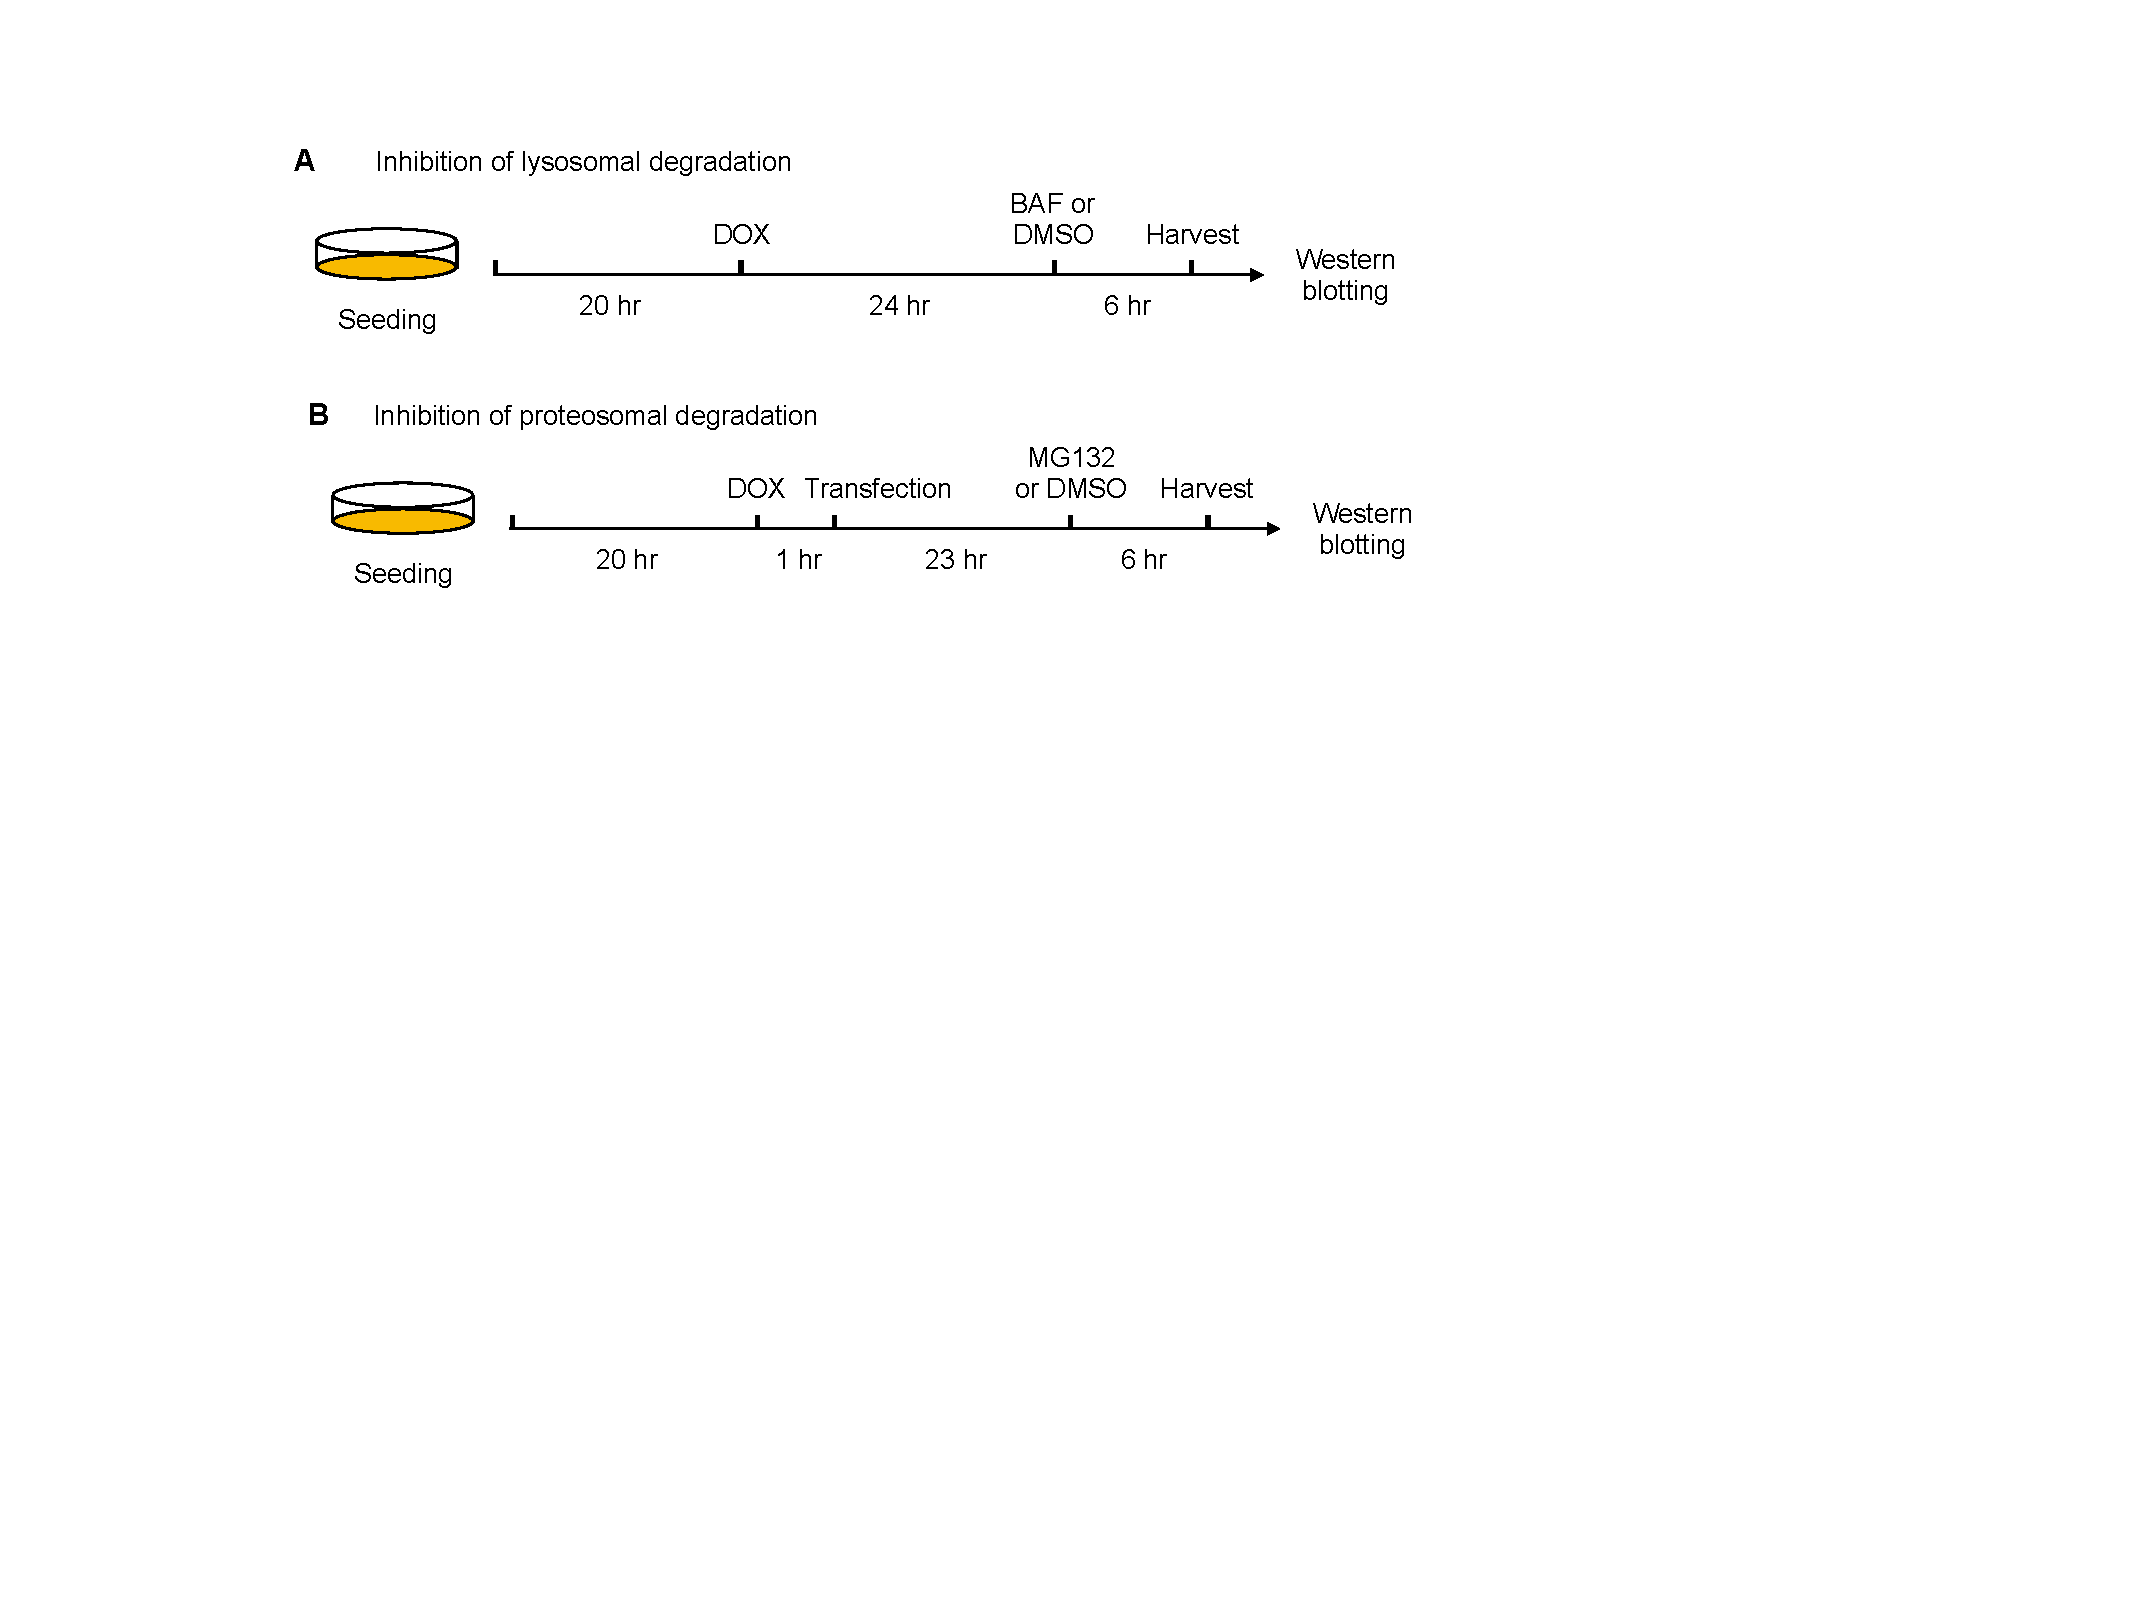
\includegraphics[scale=0.7]{Figures/treatment}
\caption{A timeline of inhibition experiments.}
\label{fig:inhibition}
\end{figure}
\normalfont Inhibitor treatment experiments were performed as the doxycycline (DOX) induction experiments but only with the 24 hr induction time point. In addition to inducing GLUT1 expression with 0.1 \textmu g/mL doxycycline, different inhibitors or DMSO (Biomol) control were added. Lysosomal degradation was inhibited using 250 nM bafilomycin A1 (Invitrogen, BAF) in DMSO for 6 hr before the cells were lysed for Western blotting analysis (Figure~\ref{fig:inhibition} A).

Cells for proteosomal inhibition experiments were transfected with UL21a-HA, an HA-epitope tagged HCMV gene, 1 hr after adding doxycycline. In brief, 20 \textmu g UL21a-HA was mixed with 40 \textmu L jetPRIME (Polyplus) in 2 mL jetPRIME (Polyplus) buffer. After incubation for 10 min, 200 \textmu L of the resulting transfection mix was added drop wise onto the cells in each well. On the next day proteasomes were blocked using 20 mM MG132 (Cayman chemical) in DMSO for 6 hr. The cells were then lysed for Western blotting analysis (Figure~\ref{fig:inhibition} B). The cellular levels of UL21a were taken as the positive control for the inhibitory effect of MG132 treatment.
\\
\\*
\bfseries{BioID and mass spectrometry analysis}\\
\normalfont Cells scraped from 15 cm plates were spun down at 300 rcf at \SI{4}{\celsius} for 4 min. After resuspension in ice-cold PBS, the triple SILAC labels were combined into a forward and a reverse experiment (Figure~\ref{fig:bioid}). The cells were spun down again and the cell pellets were resuspended in 1.5 mL of RIPA buffer (50 mM tris-HCl, 150 mM NaCl, 1\% NP-40, 1 mM EDTA, 1 mM EGTA, 0.1\% SDS, 1\% sodium deoxycholate, pH 7.5, supplemented with 75 Units/mL benzonase and protease inhibitors). After incubation with agitation at \SI{4}{\celsius} for 1 hr, the lysates were sonicated on ice for 3 min. The lysates were then centrifuged for 20 min at 16 100 rcf at \SI{4}{\celsius} to remove cell debris and the supernatants were transferred to 2 mL Eppendorf tubes.

For affinity purification a 180 {}\textmu L bed volume of streptavidin T1 magnetic beads (Invitrogen) was washed in PBS twice and RIPA buffer once before being resuspended in 200 {}\textmu L RIPA buffer. 100 {}\textmu L of the bead solution was added to each lysate sample. Affinity purification was performed at \SI{4}{\celsius} for 3 hr on a rotating wheel.

The beads were then carefully washed twice in RIPA buffer and twice in TAP lysis buffer (50 mM HEPES-KOH, 100 mM KCl, 10\% glycerol, 2 mM EDTA, 0.1\% NP-40, pH 8.0). The detergents were removed by washing three times in 50 mM ABC. The beads were resuspended in 200 {}\textmu L ABC and 10 {}\textmu L of 10 mM DTT in 50 mM ABC was added to reduce disulfide bonds of proteins. After 30 min incubation in a thermomixer at \SI{30}{\celsius} at 500 rpm, 10 {}\textmu L of 55 mM IAA (Sigma-Aldrich) in 50 mM ABC was added to alkylate the cysteine residues and the samples were incubated in the dark at \SI{30}{\celsius} at 500 rpm for 30 min. The samples then were digested with 1.5 {}\textmu g trypsin (Promega) and incubated overnight at \SI{30}{\celsius} at 1100 rpm. On the next day, the tryptic peptides were separated from beads with a magnetic rack and transferred to fresh 1.5 mL tubes. The digestion was stopped by acidification with 10 \textmu L of 10\% TFA and the tryptic peptides were loaded on C18 StageTip columns for purification~\cite{Rappsilber}. After washing with sample buffer (3\% TFA, 5\% acetonitrile) twice, the peptides were eluted from the columns into an autosampler plate with 50 {}\textmu L buffer B (0,1\% formic acid, 80\% acetonitrile). A vacuum centrifuge (Eppendorf) was used to evaporate the solvent and 10 {}\textmu L buffer A (5\% acetonitrile, 0,1\% formic acid) was added to the samples.

Peptides were separated on a reverse-phase column on a High Performance Liquid Chromatography (HPLC) system (ThermoScientific) with a gradient set up as the following ratios of buffer B in buffer A: 2 min at 250 {}\textmu L/min with a linear gradient from 5\% to 6\% buffer B, 18 min at 200 {}\textmu L/min from 6\% to 8\%, 80 min at 200 {}\textmu L/min from 8\% to 20\%, 80 min at 200 {}\textmu L/min from 20\% to 33\%, 20 min at 200 {}\textmu L/min from 33\% to 45\%, 2 min at 200 {}\textmu L/min from 45\% to 60\%, 1 min at 250 {}\textmu L/min from 60\% to 95\%, 5 min at 250 {}\textmu L/min with 95\% buffer B, 1 min at 250 {}\textmu L/min from 95\% to 75\%, and 5 min at 250 {}\textmu L/min at 75\% buffer B. Peptides were ionized using an electrospray ionization source (ThermoScientific) and analyzed on a Q-Exactive Plus Orbitrap instrument (ThermoScientific). The mass spectrometer was operated with Xcalibur in data-dependent acquisition mode with the following parameters: a full MS scan (resolution: 70 000, scan range: 300 to 1700 m/z, AGC target: 1 000 000 ions, maximum injection time: 120 ms) followed by MS-MS analysis (resolution: 17 500, AGC target: 100 000 ions, maximum injection time: 60 ms) on the top 10 abundant ions.

The resulting raw files were analyzed using MaxQuant 1.5.2.8~\cite{Cox}. The reference human proteome database, consisting of 159 616 entries, was downloaded from the UniProt Knowledgebase on February 28th, 2017. Lys4, Arg6 and Lys8, Arg10 were added to the labels. Variable modifications were set as N-terminal acetylation and oxidation of methionines. The \textit{in silico} digestion of peptides in the reference database was performed with trypsin/P site-specific cleavage. Default global parameters were kept except that "re-quantify" and "match between runs" were turned on. The false discovery rate, assessed by in-parallel searching in a decoy database generated by reversing the reference database, was set to 0.01 at peptide and protein levels. 

The following analysis was performed using Perseus v1.5.8.4 and R v3.3.3~\cite{Tyanova}. The proteins identified from the reverse database, potential contaminants and proteins identified only by a modification site were removed. The intensities and ratios were logarithmized (base 10 and 2, respectively). To determine specific proximity interactions, only proteins whose H/L and M/L fold changes were larger than 1.5 in both forward and reverse experiments were kept for further analysis. Metascape was used for GO enrichment analysis~\cite{Tripathi}.
\\
\\*
\bfseries{Transferrin uptake}\\
\normalfont After 24 hr of doxycycline induction, the cells were starved for 1 hr in starvation buffer [serum-free medium supplemented with 20 mM HEPES (Life Technologies)]. Transferrin conjugated with Alexa Fluor 568 (Life Technologies) was diluted in starvation buffer to a final concentration of 10 {}\textmu g/mL and droplets of 35 {}\textmu L transferrin solution were pipetted onto a parafilm in a dark humid chamber. The coverslips were then carefully lifted off the bottom of the plate with forceps and placed face-down on the droplets. The humid chamber was incubated at \SI{37}{\celsius} and 5\% CO\textsubscript{2} for 10 min. After transferrin uptake, the coverslips were washed 3 times for 5 min with PBS supplemented with 10 mM MgCl\textsubscript{2} and 10 mM CaCl\textsubscript{2}, followed by standard immunostaining procedures described as below.
\\
\\*
\bfseries{Immunostaining and confocal microscopy}\\
\normalfont Prior to staining, cell culture medium was aspirated and cells were briefly washed with pre-warmed PBS. The cells were fixed in 4\% PFA for 15 min at room temperature before being washed 3 times for 5 min in PBS. To permeabilize cells and block unspecific binding sites the cells were incubated for 1 hr at room temperature in blocking buffer [5\% goat serum (Sigma-Aldrich), 0.3\% Triton X-100 (Sigma-Aldrich) in PBS]. The primary antibody was diluted in antibody dilution buffer [1\% BSA - Fraction V (Sigma-Aldrich), 0.3\% Triton X-100 in PBS], as indicated in Table~\ref{tab:IF}. The coverslips were placed face-down on droplets of 50 {}\textmu L primary antibody solution on a piece of parafilm in a dark humid chamber. After 1 hr incubation at room temperature, the coverslips were placed face-up in the plate and washed 3 times for 5 min in PBS. Similarly, the coverslips were incubated with secondary antibody solution for 1 hr at room temperature in the humid chamber before being washed for 5 min in PBS. The coverslips were then counterstained with DAPI (0.1 {}\textmu g/mL in PBS, Sigma-Aldrich) for 3 min and washed for 10 min in PBS. Finally, the coverslips were briefly rinsed in Milli-Q H\textsubscript{2}O and mounted with ProLong Gold Antifade Mountant (Life Technologies) on slides. After overnight incubation, the slides were stored at \SI{4}{\celsius} in the dark.

\begin{table}[h]
%\captionsetup{font=normalsize}
\caption{Antibodies for immunofluorescence and their dilutions.}
\label{tab:IF}
\small
\centering
\begin{tabular*}{\textwidth}{l@{\extracolsep{\fill}}lll}
\toprule
\tabhead{Antibodies} & \tabhead{Source} & \tabhead{Dilution} & \tabhead{Conjugate}\\
\midrule
Mouse monoclonal anti-FLAG & Sigma-Aldrich & 1:200 & \\
Rabbit polyclonal anti-GLUT1 & Merck Millipore & 1:500 & \\
Rabbit monoclonal anti-EEA1 & Cell Signaling Technology & 1:100 & \\
Rabbit monoclonal anti-Rab4 & Cell Signaling Technology & 1:100 & \\
Rabbit monoclonal anti-Rab9 & Cell Signaling Technology & 1:100 & \\
Rabbit monoclonal anti-Rab11 & Cell Signaling Technology & 1:100 & \\
Rabbit monoclonal anti-LAMP1 & Cell Signaling Technology & 1:100 & \\
Mouse monoclonal anti-Vti1a & BD Biosciences & 1:100\\
Mouse monoclonal anti-Vti1b & BD Biosciences & 1:100\\
Mouse monoclonal anti-STX6 & BD Biosciences & 1:100\\
Goat anti-mouse IgG (H+L) & Invitrogen & 1:500 & Alexa Fluor 488\\
Goat anti-rabbit IgG (H+L) & Invitrogen & 1:500 & Alexa Fluor 488\\
Donkey anti-rabbit IgG (H+L) & Invitrogen & 1:500 & Alexa Fluor 568\\
Donkey anti-mouse IgG (H+L) & Invitrogen & 1:500 & Alexa Fluor 568\\
\bottomrule
\end{tabular*}
\end{table}
Images in this thesis were acquired using Leica DMI6600 confocal laser scanning microscope with an HCX PL APO 63.0$\times$/1.40 oil objective and Leica Application Suite Advanced Fluorescence (v2.7.3 build 9725) software. As summarized in Table~\ref{tab:laser}, fluorophores were excited using 405 nm laser diode, Argon 488 nm laser (20\% power) or DPSS 561 nm laser and detected using photomultiplier tubes (PMT). The pinhole diameter was set to 95.6 {}\textmu m, scanning mode was unidirectional, line average was 2, sampling speed was 400 Hz. For co-localization studies the zoom was set to 5 and the voxel size was 48.1 nm (width) $\times$ 48.1 nm (height) $\times$ 125.9 nm (depth). The regions for imaging were selected by choosing cells with good DAPI staining.

\begin{table}[h]
%\captionsetup{font=normalsize}
\caption{Settings for fluorescence excitation and detection.}
\label{tab:laser}
\small
\centering
\begin{tabular*}{\textwidth}{l@{\extracolsep{\fill}}lllll}
\toprule
\tabhead{Fluorophore} & \tabhead{Laser line} & \tabhead{Laser intensity} & \tabhead{PMT} & \tabhead{PMT gain} & \tabhead{PMT offset}\\
\midrule
DAPI & 405 nm & 8.00\% & 413-477 nm & 619 V & -1\\
Alexa 488 & 488 nm & 12.00\% & 506-598 nm & 646 V & -1\\
Alexa 568 & 561 nm & 15.00\% & 580-710 nm & 619 V & -1\\
\bottomrule
\end{tabular*}
\end{table}
The z-stack confocal microscopy images were further analyzed using ImageJ v1.51j. The stack viewing and color options were set as the default configuration of the Bio-Formats plugin. One z slice was selected in each image to represent all stacks. The background was uniformly adjusted in each staining experiment whereas the contrast was individually adjusted in each image. 

Imaris v8.4.1 was used for the quantitative colocalization analysis. The original z-stack images were adjusted by adding an adequate mask on the green channel to subtract background noise~\cite{Costes}. The threshold for the mask was uniformly adjusted in each staining experiment. Cells without FLAG staining were cropped out. Automatic thresholding was used to define the area where a colocalization would be determined and the statistics was calculated for each colocalization channel~\cite{Costes}. For the images whose observed correlation was not statistically significant in comparison to randomized images, the colocalization channel was built without additional thresholding on the masked dataset. The resulting thresholded Pearson's and Mander's coefficients were exported. 
%----------------------------------------------------------------------------------------

% Define some commands to keep the formatting separated from the content 
